\documentclass[tikz,border=5mm]{standalone}
\usepackage{tikz}
\usetikzlibrary{shapes.geometric, positioning}

\begin{document}
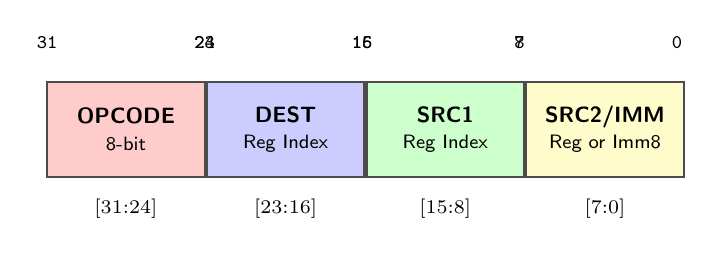
\begin{tikzpicture}[
    font=\sffamily\small,
    field/.style={
        rectangle,
        draw=black!70,
        thick,
        minimum height=1.2cm,
        align=center,
        font=\sffamily\footnotesize
    }
]
    % Define field widths (8 bits each = 2cm per field)
    \def\fieldwidth{2.0cm}
    
    % Bit position labels (top)
    \node[font=\scriptsize\ttfamily, anchor=south] at (0, 1.5) {31};
    \node[font=\scriptsize\ttfamily, anchor=south] at (2, 1.5) {24};
    \node[font=\scriptsize\ttfamily, anchor=south] at (2, 1.5) {23};
    \node[font=\scriptsize\ttfamily, anchor=south] at (4, 1.5) {16};
    \node[font=\scriptsize\ttfamily, anchor=south] at (4, 1.5) {15};
    \node[font=\scriptsize\ttfamily, anchor=south] at (6, 1.5) {8};
    \node[font=\scriptsize\ttfamily, anchor=south] at (6, 1.5) {7};
    \node[font=\scriptsize\ttfamily, anchor=south] at (8, 1.5) {0};
    
    % Field boxes with colors
    \node[field, fill=red!20, minimum width=\fieldwidth] (opcode) at (1, 0.6) {\textbf{OPCODE}\\ \scriptsize 8-bit};
    \node[field, fill=blue!20, minimum width=\fieldwidth, right=0cm of opcode] (dest) {\textbf{DEST}\\ \scriptsize Reg Index};
    \node[field, fill=green!20, minimum width=\fieldwidth, right=0cm of dest] (src1) {\textbf{SRC1}\\ \scriptsize Reg Index};
    \node[field, fill=yellow!20, minimum width=\fieldwidth, right=0cm of src1] (src2) {\textbf{SRC2/IMM}\\ \scriptsize Reg or Imm8};
    
    % Bit range labels (bottom)
    \node[font=\scriptsize, below=0.15cm of opcode] {[31:24]};
    \node[font=\scriptsize, below=0.15cm of dest] {[23:16]};
    \node[font=\scriptsize, below=0.15cm of src1] {[15:8]};
    \node[font=\scriptsize, below=0.15cm of src2] {[7:0]};
    
\end{tikzpicture}
\end{document}
